%\documentclass[18pt,oneside,a4paper, titlepage]{article}

%\usepackage[hidelinks]{hyperref}
%\usepackage[pdftex]{graphicx}

%\begin{document}

\newpage
	\section{Architectural Design}
		\subsection{Overview}
				
\newpage
		\subsection{High level components and their interaction}
		% here you can introduce the high level components of your architecture (in our basic example in the slides about design you find these in slide 7) and describe the main interaction between them (no details here. You can say why some components talk to each other, why, if the communication is synchronous or asynchronous, any other info you think is useful at this point). 
			\vspace{1cm}
			\begin{figure}[h]
				\centering
				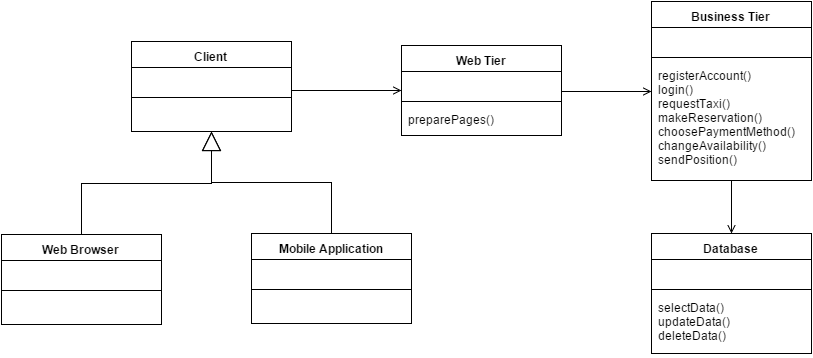
\includegraphics[scale=0.45]{HighLevelComp.png}
			\end{figure}
			\vspace{1cm}
			\begin{itemize}
				\item \textbf{Client}: this part runs on the client devices via a Web browser or the mobile application. It allows the users to insert and submit the data in the input forms, that are sent to the application server. On the other hand, the taxi drivers can send information about their availability to the server and the application client monitors their GPS position in order to move the taxi drivers to another queue if they change their area. 
				\item \textbf{Application Server}: this part runs on the JEE server. It is composed of a web server part, which always listens to all the clients requests and is responsible for the creation of the faces and pages of the client interfaces. The application server, instead, contains the logical part of the application, collecting and managing the information from the clients and the database. In fact, it analyses the data coming from the clients and, according to the requests, it modifies or asks for the required information stored in the database, then it is able to answer the client request, sending it the result.  
				\item \textbf{Database}: this part contains the database where all the application data are stored. It is not only accessed by the application server, but also by the administrators, who can, for example, directly add a taxi driver account to the database. 
			\end{itemize}	
			
	\newpage
		\subsection{Component view}
		% here you have a refinement of what you have in Section 4.B and identify sub-components. For instance, the diagram in slide 6 could be a diagram showing a  component view
		These are the components that define the myTaxiService system architecture. The system is composed by many subsystems 
	\newpage	
		\subsection{Deployment view}
		% this is what you have in slide 8, that is, the identification of the artifact that need to be deployed to have the system working
	\newpage
		\subsection{Runtime view}
		%	You can use sequence diagrams to describe the way components interact to accomplish specific tasks typically related to your use cases
		% this is what you have in slide 9 plus sequence diagrams describing the way components behave in order to accomplish a certain activity
	\newpage
		\subsection{Component interfaces}
		% here you define the interfaces of your components, that is, which operations they offer to the external world, their meaning, any input and output parameter (name, possible set of values/type)
		Here is presented a list of the interfaces defined in the component diagram and their functionalities.
		\begin{itemize}
			\item \textbf{Access.}
			\item \textbf{TaxiDriverArea.}
			\item \textbf{PassengerArea.}
			\item \textbf{RequestTaxiVisitor.}
			\item \textbf{RequestTaxiPassenger.}
			\item \textbf{MakeReservation.}
			\item \textbf{PaymentMethod.}
		\end{itemize}
	\newpage
		\subsection{Selected architectural styles and patterns}
		%	Please explain which style/patterns you used, why and how
		\begin{itemize}
			\item \textbf{Client/Server.} The client/server architecture is the optimal solution for the myTaxiService system, as it is necessary to have a central system that listens, manages and forwards the requests of the different clients. There is a central server that contains the logic of the application and the clients are the users of the system, such as visitors, passengers and taxi drivers.
			\item \textbf{Three-tier.} It has been adopted a three-tier architectural model, composed by thin client, application server and database.\\ This architecture is the best choice for our system, even if it has some cons, such as the complexity of the structure and the difficulty of set up and maintenance, it still has several pros. For example, it guarantees increased performance and great flexibility, useful if there will be any future change concerning the architecture. Moreover it is granted a great security level, thanks to the decoupling of logic, data and presentation, which is essential as the system deals with several personal data.
			\item \textbf{Event-Based System.} The myTaxiService application is based on the event firing %triggering?
			. \\It is necessary, in fact, that the system is reactive and that does different quick operations according to the action of the clients. For example the visitors and passengers make requests and reservations, which the system has to manage and forward to the first taxi of the area, and the taxi drivers can change their availability state and the system has to start or end the monitoring of their position, and they can accept or decline a request and the system has to manage the queue. \\The users and the taxi drivers are registered to different events and expect to receive notifications about what they need, whether it is the arrival of a taxi or the requests of the users.\\ The events are asynchronous and based on a "send and forget" paradigm, where the system only cares for sending the notifications to the designated clients or doing the actions needed in response of the event fired.
			\item  \textbf{Service Oriented Architecture.} A service-oriented architecture is necessary if the system wants to be more flexible and expandable. In fact, the myTaxiService application needs to provide programmatic interfaces in order to be open to future implementations of additional services. This can be guaranteed with this architectural choice, which is based on the loose coupling of the services, allowing to easily add more functionalities, without starting from scratch when a change is needed, and to simplify the maintenance of the system.
		\end{itemize}
							
%\end{document}